% Document class and import any packages that are used.
\documentclass[12pt,titlepage]{article}
\pagestyle{plain}
\usepackage[utf8]{inputenc}
\usepackage[empty]{fullpage}
\usepackage[a4paper,margin=1in, headsep=24pt, headheight=2cm]{geometry}
\usepackage{enumitem}
\usepackage{hyperref}
\usepackage{setspace}
\usepackage{indentfirst}
\usepackage{wrapfig}
\usepackage{natbib}
\usepackage{multirow}
\usepackage{titling}
\usepackage{fancyhdr}
\usepackage{graphicx}
\usepackage{titlesec}

% Set section format
\titleformat{\section}
  {\normalfont\normalsize\bfseries\itshape}{\thesection.}{1em}{}
  
\titleformat{\subsection}
  {\normalfont\normalsize\itshape}{\thesubsection.}{1em}{}

\begin{document}

% Set page style and layout style.
\begin{titlepage}
\title{Rhetoric of Climate Change Discourse on Twitter}
\author{Nianhui Guo (1005205779), Jolene Milne (1006310902),\\
Robin Thapa (1007040355), Ryan Wong (1004438156)\\
CCT416 Social Data Analytics\\
Dr. Radha Maharaj\\
Institute of Communication, Culture, Information and Technology\\
University of Toronto Mississauga\\}
\date{4 April 2023}
\maketitle
\end{titlepage}

\newpage
\tableofcontents
\setcounter{secnumdepth}{0}

\newpage
\begin{center}
    \textbf{\Large Rhetoric of Climate Change Discourse on Twitter}
\end{center}

\begin{table}[ht!]
\centering
  \begin{tabular}{lllll}
  & precision & recall & f1-score & support \\ \hline
negative     & 0.68      & 0.66   & 0.67     & 343     \\
neutral      & 0.25      & 0.03   & 0.05     & 39      \\
positive     & 0.69      & 0.77   & 0.72     & 391     \\
             &           &        &          &         \\
accuracy     &           &        & 0.68     & 733     \\
macro avg    & 0.54      & 0.48   & 0.48     & 733     \\
weighted avg & 0.66      & 0.68   & 0.67     & 733    
  \end{tabular}
  \caption{SVM Classification Report Summary}
  \label{tab:svm}
\end{table}

\singlespacing

\section{Introduction}
The topic we chose is climate change. Our motivation was a curiosity behind the types of discussions, thoughts and opinions on climate change that social media users post online. More specifically, we wanted to discover what the average user is posting about climate change, and the general opinions/information that is circulating among various circles of social media based on the topic of climate change. Generally, we have noticed and are curious about how people, either online or offline, hold a variety of differing opinions on climate change. Many of these people may agree with and support climate change evidence, while the others are more skeptical and may doubt or deny it. This is the source of our questioning; how many people on social media support climate change, and also, how many deny it? What are the types of words people use to support/justify their own opinions? We are also curious about the possibility of misinformation being spread across social media, and how this may influence climate change discussions. Where do people’s social media posts source their points/evidence from? For this goal, we have used and compared various methods of data collection and sentiment analysis to answer our questions as accurately as possible. The results of this analysis display the variety of user opinion and the most common sentiments/topics resulting from the data collection, bringing us closer to our goals.

\newpage
\section{Methodology}

\phantomsection
\subsection{Pre-processing}


\newpage
\section{Observations}
Based on the description above, our research process began with preprocessing the collected data. We then tested three lexicon-based sentiment analysis approaches on the processed data: TextBlob, NLTK-SentiWord, and VADER. Upon evaluating their performance and practicality, we determined that VADER was the most suitable lexicon-based method for our study. Additionally, we refined a portion of the processed data to experiment with two machine learning sentiment analysis approaches, namely Naive Bayes and SVM. By examining their predicted sentiment labels graph, confusion matrix, and precision scores, we found that both models had similar accuracy rates. Therefore, we increased our research sample size to 10,000 tweets and discovered that the SVM model performed better, with lower error rates and higher accuracy. Finally, to verify the accuracy of our results, we compared and analyzed the final images obtained using the VADER lexicon-based approach and the SVM machine learning approach, finding that both approaches produced very similar image structures.

Sentiment Analysis - TextBlob
The graph shows that positive sentiment tweets range from 140 to 160, neutral sentiment tweets range from 100 to 120, and negative sentiment tweets range from 80 to 100. positive tweets outnumber neutral and negative tweets, with a gap of 20 tweets between the latter two. A more pronounced gap of 40 tweets existed between neutral and positive tweets. The greatest gap, about 60 tweets, was between the highest number of the positive and minimum number of the negative tweets.

Sentiment Analysis - SentiWord
The graph illustrates that positive sentiment tweets range from 140 to 160, negative sentiment tweets from 120 to 140, and neutral sentiment tweets at around 60. Positive sentiment tweets slightly outnumber negative tweets, followed by neutral tweets. Positive and negative tweet quantities are similar, with a 20-tweet difference, while negative and neutral tweet quantities differ by nearly 70 tweets. The gap between the highest (positive sentiment) and lowest (neutral sentiment) tweet counts is about 90 tweets, more pronounced than in the TextBlob results.

Sentiment Analysis - VADER
In the graph, positive sentiment tweet counts are around 140, negative sentiment tweet counts are approximately 110, and neutral sentiment tweet counts are estimated at 10 or even fewer. Further analysis reveals a 30-tweet gap between positive and negative sentiment tweet counts. The difference between negative and neutral sentiment tweet counts is much larger, nearly 100 tweets. Lastly, there's a nearly 130-tweet gap between the highest (positive sentiment) and lowest (neutral sentiment) tweet counts, making VADER's results more distinct and having the largest gap compared to TextBlob and SentiWord.

Predicted Sentiment Analysis with 1000 Tweets - Naive Bayes 
The bar chart shows that positive sentiment tweets are around 150, negative sentiment tweets are approximately 105, and neutral sentiment tweets are about 5. There is a difference of roughly 45 tweets between the highest positive sentiment tweets and the second-highest negative sentiment tweets. However, a more significant gap of approximately 100 tweets exists between the second-highest negative sentiment tweets and the lowest neutral sentiment tweets.

Predicted Sentiment Analysis with 1000 Tweets - SVM
The bar chart displays approximately 150 positive sentiment tweets, 100 negative sentiment tweets, and around 10 neutral sentiment tweets. Upon closer examination, the difference between the highest number of positive sentiment tweets and negative sentiment tweets is about 50 tweets, while the gap between negative sentiment and neutral sentiment tweets is roughly 90 tweets.

figure~\ref{fig:top10}

figure~\ref{fig:tfidf}

\begin{figure}[!ht]
  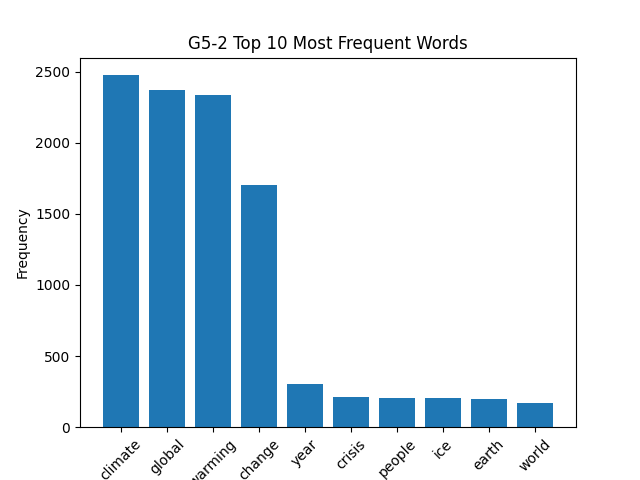
\includegraphics[width=6in]{G5-2_FrequentTop10.png}
  \caption{sample text}
  \label{fig:top10}
\end{figure}

\begin{figure}[!ht]
  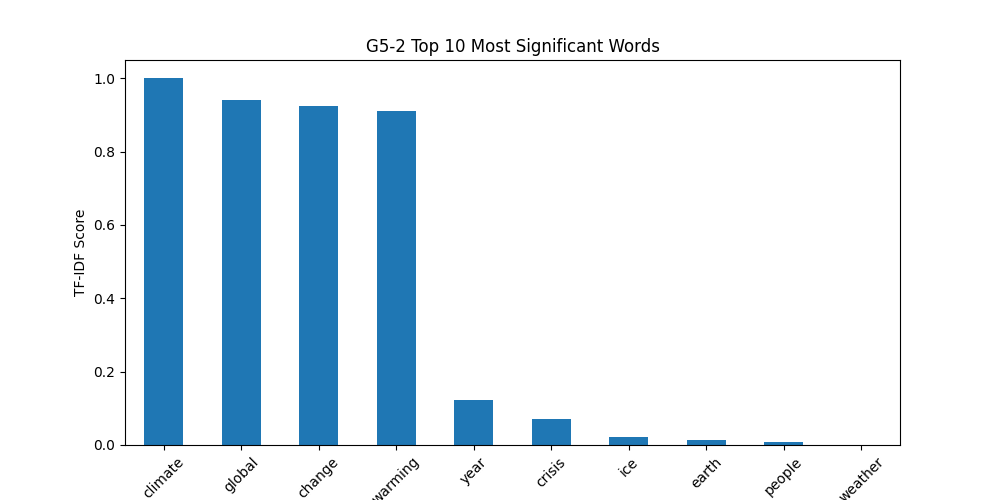
\includegraphics[width=6in]{G5-2_TF-IDF.png}
  \caption{sample text}
  \label{fig:tfidf}
\end{figure}


\newpage
\section{Discussion}


\newpage
\section{Conclusion}

\citep{harvey2018internet}
\citep{jost2019positive}


\newpage
\bibliographystyle{apalike}
\bibliography{references}

\end{document}